\documentclass{standalone}

\usepackage{amsmath}
\usepackage{tikz}
\usetikzlibrary{arrows.meta, positioning, calc}

% Respect chosen fonts (serif) and metrics
\renewcommand{\familydefault}{\rmdefault}

%% font
\usepackage{dsfont}
\usepackage[T1]{fontenc}
\usepackage{lmodern}
\usepackage{amsmath}

\begin{document}

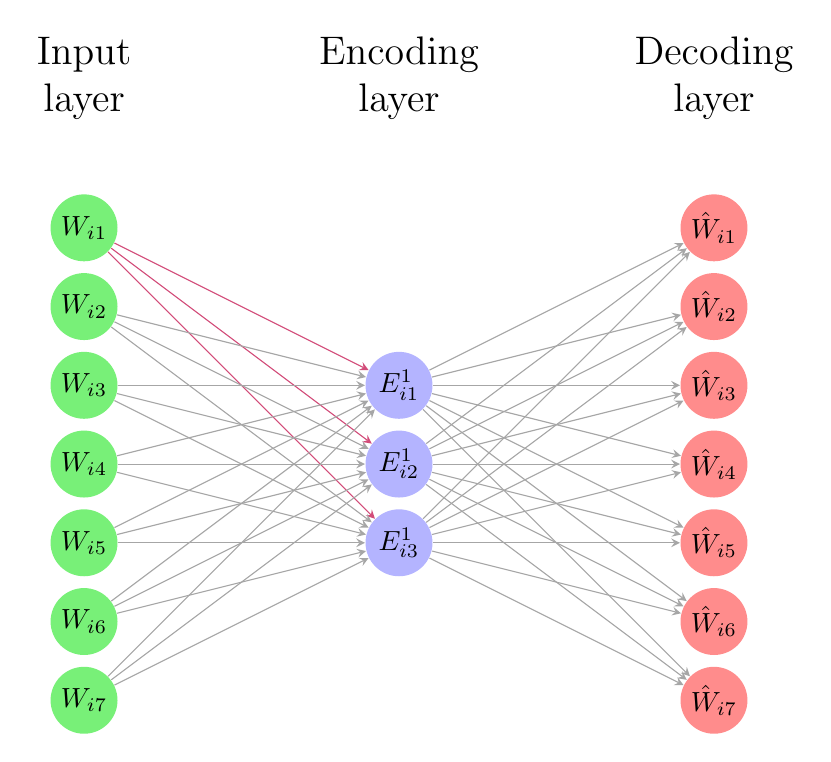
\begin{tikzpicture}[x=1cm,y=1cm,>=stealth]

% Titles
\node[font=\Large] at (0,8) {Input};
\node[font=\Large] at (0,7.4) {layer};

\node[font=\Large] at (4,8) {Encoding};
\node[font=\Large] at (4,7.4) {layer};

\node[font=\Large] at (8,8) {Decoding};
\node[font=\Large] at (8,7.4) {layer};

% Colors
\definecolor{inputgreen}{RGB}{120,240,120}
\definecolor{hiddenblue}{RGB}{180,180,255}
\definecolor{outputred}{RGB}{255,140,140}

% Input nodes
\foreach \i/\y in {1/5.8,2/4.8,3/3.8,4/2.8,5/1.8,6/0.8,7/-0.2} {
    \node[circle, fill=inputgreen, minimum size=0.85cm, inner sep=0pt] (I\i) at (0,\y) {$W_{i\i}$};
}

% Hidden nodes
\foreach \j/\y in {1/3.8,2/2.8,3/1.8} {
    \node[circle, fill=hiddenblue, minimum size=0.85cm, inner sep=0pt] (H\j) at (4,\y) {$E^{1}_{i\j}$};
}

% Output nodes
\foreach \i/\y in {1/5.8,2/4.8,3/3.8,4/2.8,5/1.8,6/0.8,7/-0.2} {
    \node[circle, fill=outputred, minimum size=0.85cm, inner sep=0pt] (O\i) at (8,\y) {$\hat{W}_{i\i}$};
}

% Connections: input -> hidden

\foreach \i in {1} {
    \foreach \j in {1,...,3} {
        \draw[purple!70,->,thin] (I\i) -- (H\j);
    }
}

\foreach \i in {2,...,7} {
    \foreach \j in {1,...,3} {
        \draw[gray!70,->,thin] (I\i) -- (H\j);
    }
}

% Connections: hidden -> output
\foreach \j in {1,...,3} {
    \foreach \i in {1,...,7} {
        \draw[gray!70,->,thin] (H\j) -- (O\i);
    }
}

\end{tikzpicture}

\end{document}